% BEGIN PREAMBEL
\documentclass[9pt]{beamer}
\usepackage[british]{babel}
\usepackage{multimedia}
\usepackage{amsmath,amsfonts,amssymb}
\usepackage{upgreek}
\usepackage{pgfpages}
\usepackage[version=3]{mhchem}
\usepackage{lmodern}
\usepackage{graphicx}
\usepackage{multicol}
\usepackage{color}
\usepackage{xcolor,fontawesome}
\usepackage{wrapfig}
\usepackage{siunitx}
\usepackage{fontspec}
\usepackage{tikz}
\usepackage{textpos}
\usepackage{booktabs}
\usepackage{subcaption}
\usepackage{wasysym}
\newfontfamily\ubuntu{Ubuntu}
\newcommand{\as}{\\[14pt]}
\newcommand{\s}{\\[7pt]}
\newcommand{\is}{\\[2pt]}
\newcommand{\no}{\noindent}
\newcommand{\ka}{\hspace*{0.5cm}}
\newcommand{\ma}{\hspace*{1cm}}
\newcommand{\ga}{\hspace*{1.5cm}}
\newcommand{\li}{\left|}
\newcommand{\re}{\right|}
\newcommand{\const}{\text{const.}}
\newcommand{\z}{\text}
\newcommand{\terminal}[1]{\colorbox{black}{\textcolor{white}{{\fontfamily{phv}\selectfont \scriptsize{#1}}}}}
\newcommand{\plugin}[1]{\textit{\flq#1\frq}}
\newcommand{\ra}{$\rightarrow$ }
\definecolor{cadmiumgreen}{rgb}{0.0, 0.42, 0.24}
\usetheme{Boadilla}
\graphicspath{ {Pics/} }
\makeatletter
\def\input@path{ {sections/} }
\makeatother
\usecolortheme{beaver}
\useoutertheme{miniframes}
\beamertemplatenavigationsymbolsempty
\makeindex
\title[Diamond Beam Tests]{Beam Tests Investigating Diamond as Detector Material}
\author[M. Reichmann]{Michael Reichmann}
\institute[\textbf{\textit{ETH}}\scalebox{.6}{\textit{Z\"{u}rich}}]{Swiss Federal Institute of Technology Zurich}
\AtBeginSection{\frame{\sectionpage}}
% END PREAMBEL

\begin{document}

% ============= TITLE PAGE =============
\usebackgroundtemplate{\tikz\node[opacity=0.2] {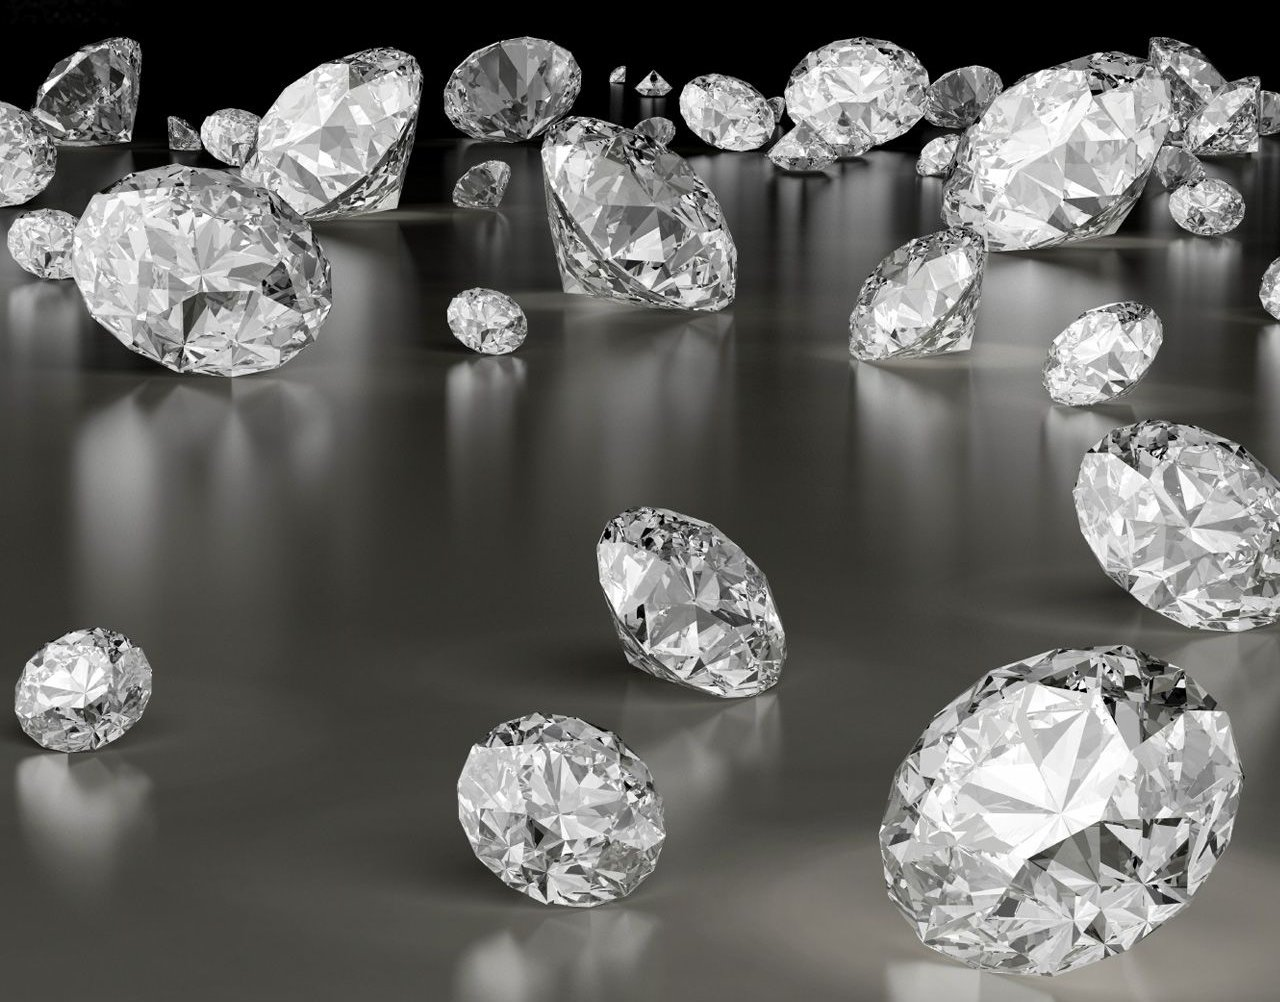
\includegraphics[height=\paperheight,width=\paperwidth]{bkg.jpg}};}
\begin{frame}
	\begin{center}
		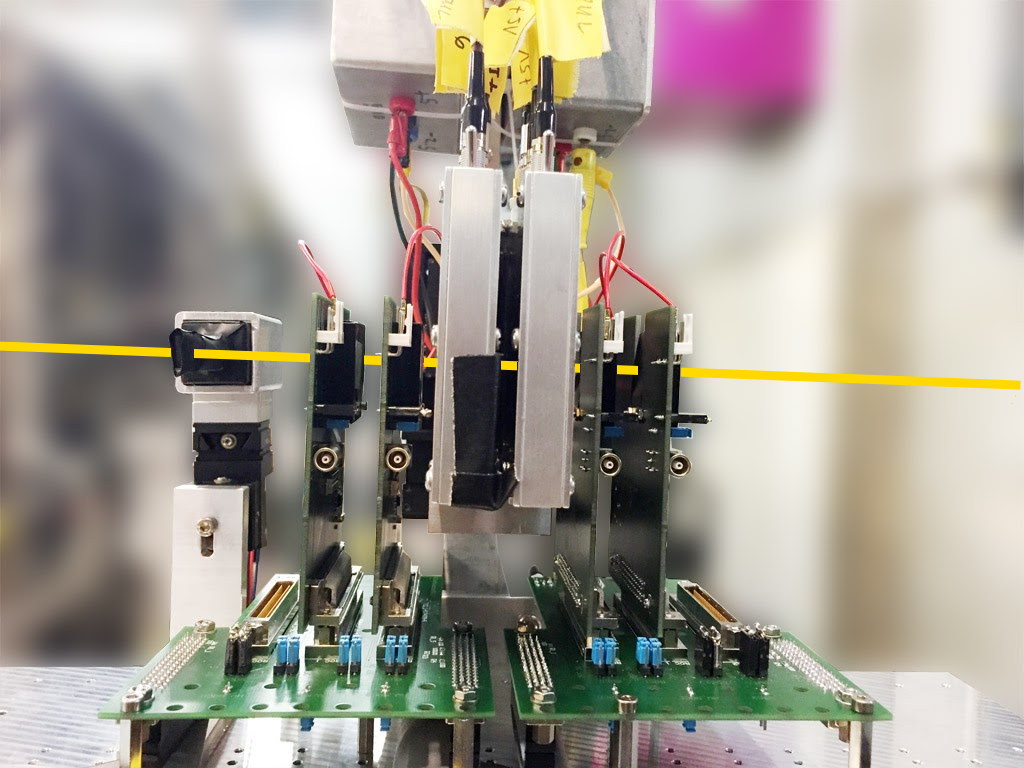
\includegraphics[width=6cm]{Setup1}
	\end{center}
	\begin{alertblock}{
		\begin{center}
			\textbf{Beam Tests Investigating Diamond as Detector Material}
		\end{center}}
		\vspace*{10pt}
		\begin{center}\small
		Michael Reichmann
		\end{center}\normalsize
	\end{alertblock}
\end{frame}
% END
\usebackgroundtemplate{}

% ============= TABLE OF CONTENTS ======
\begin{frame}[allowframebreaks]
	\frametitle{Table of contents}
	\tableofcontents   % [pausesections]
\end{frame}

% ============= MOTIVATION =============
\section{Motivation}
\begin{frame}
	\frametitle{Motivation}
	\begin{itemize}
% 		\setlength{\itemsep}{\fill}
		\item diamond as possible future material for the tracking detectors of the LHC
		\item innermost layers $\rightarrow$ highest radiation damage
		\item current detector designed to withstand \SI{250}{\per\femto\barn} of integrated luminosity
		\begin{itemize}
			\vspace*{4pt}
			\item High-Luminosity LHC: replace detector every \SI{12}{month}
		\end{itemize}
		\item \textbf{\textcolor{red}{$\rightarrow$ look for more radiation hard detector designs and/or materials}}
	\end{itemize}
	\begin{figure}
		\centering
		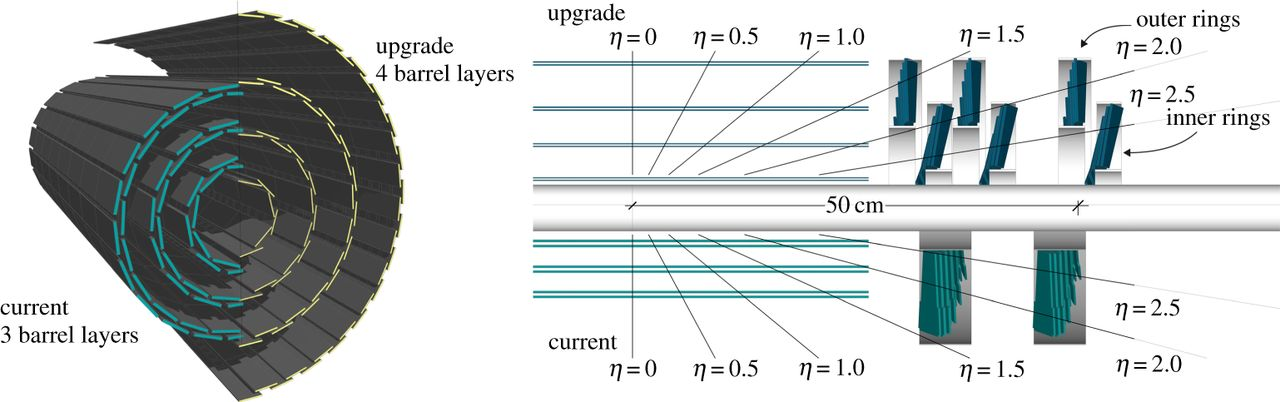
\includegraphics[width=10cm]{BPIX}
		\caption{CMS Barrel Pixel Detector upgrade with end caps}
	\end{figure}
\end{frame}

% ============= DIAMONDS ===============
\section{Diamond Detectors and Materials}
\subsection{Detector designs}
\begin{frame}
	\frametitle{Detector designs}
	\begin{itemize}
% 		\setlength{\itemsep}{\fill}
		\item Investigation of two different detector designs
		\vspace*{5pt}
		\begin{itemize}
			\item \textbf{planar diamonds}
			\begin{itemize}
				\item exchange of material
			\end{itemize}
			\item \textbf{3D diamonds}
			\begin{itemize}
				\item new type of detector
			\end{itemize}
		\end{itemize}
	\end{itemize}
	\begin{figure}[htbp] 
		\begin{center}
			\begin{subfigure}{0.45\textwidth}  
				\centering 
				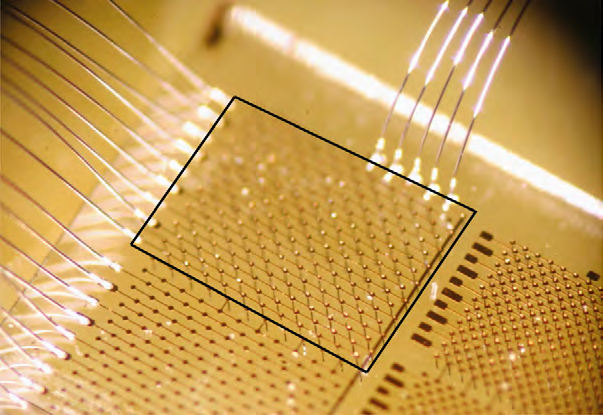
\includegraphics[height=0.4\textheight]{3D}
				\caption{prototype}
			\end{subfigure}
			\begin{subfigure}{0.45\textwidth} 
				\centering 
				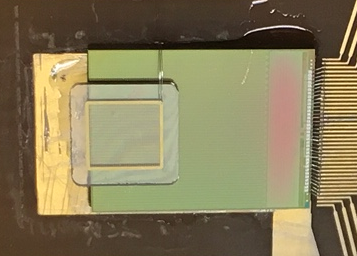
\includegraphics[height=0.4\textheight]{diapix}
				\caption{on CMS-Pixel chip} 	
			\end{subfigure} 
			\caption{3D diamond detectors} 
		\end{center}
	\end{figure}
\end{frame}
% ============== new frame
\subsection{Diamond as detector material}
\begin{frame}
	\frametitle{Diamond as detector material}
	\begin{itemize}
		\setlength{\itemsep}{\fill}
		\item \textcolor{cadmiumgreen}{$7-10$ times smaller charge loss due to radiation damage than in silicon}
		\item \textcolor{red}{signals (electrons created by a charged particle) half the size of silicon}
		\item $\rightarrow$ diamond becomes superior than silicon at a certain irradiation
		\item other advantageous properties:
		\begin{itemize}
			\item isolating material \ra negligible leakage current \ra power saving 
			\item high thermal conductivity \ra heat spreader for electronics
			\item large band gap \ra no cooling required
			\item high charge carrier mobility \ra fast signals
			\item working principle like a solid state ionisation chamber \ra no pn-junction required
		\end{itemize}
		\item disadvantages:
		\begin{itemize}
			\item high price
			\item some not fully understood behaviours 
		\end{itemize}
	\end{itemize}
\end{frame}
% ============== new frame
\subsection{Artificial diamond types}
\begin{frame}
	\frametitle{Artificial diamond types}
	\begin{itemize}
		\item used diamonds artificially grown with a chemical vapor deposition (CVD) process
		\item investigation of two different diamond types:
	\end{itemize}
	\begin{figure}[htbp] 
		\begin{center}
			\begin{subfigure}{0.45\textwidth}  
				\centering 
				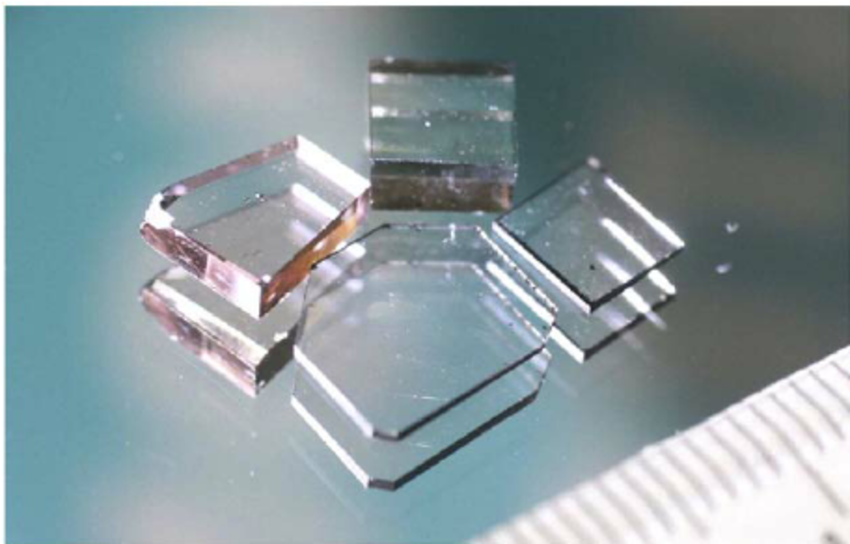
\includegraphics[height=0.4\textheight]{SCVD}
				\caption{single-crystalline CVD}
			\end{subfigure}
			\begin{subfigure}{0.45\textwidth} 
				\centering 
				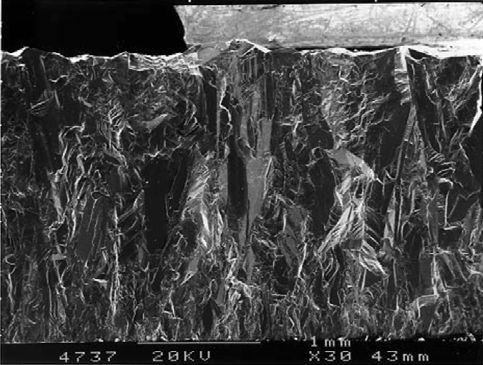
\includegraphics[height=0.4\textheight]{PCVD}
				\caption{poly-crystalline CVD} 	
			\end{subfigure} 
		\end{center}
	\end{figure}
	\begin{minipage}{5.5cm}
		\begin{itemize}
			\item grown on existing diamond crystal
			\item only small sizes (\SI{\sim.25}{cm^2})
			\item larger signals than pCVD ($5:3$)
		\end{itemize}
	\end{minipage}
	\hspace*{2pt}
	\begin{minipage}{5.5cm}
		\begin{itemize}
			\item grown on Si substrate with diamond powder
			\item large wafers (\SIrange{5}{6}{cm} \diameter)
			\item non-uniformities and grains
		\end{itemize}
	\end{minipage}
\end{frame}
% ============== new frame
\begin{frame}
	\frametitle{Diamonds in CMS}
	\begin{itemize}
		\item scCVD diamond pixel detector used in Pixel Luminosity Telescope (PLT)
		\begin{itemize}
			\vspace*{2pt}
			\item goal: stand-alone luminosity monitor for CMS
		\end{itemize}
		\item \textcolor{red}{observation of a signal dependence on incident particle rate:}
	\end{itemize}
	\begin{center}
		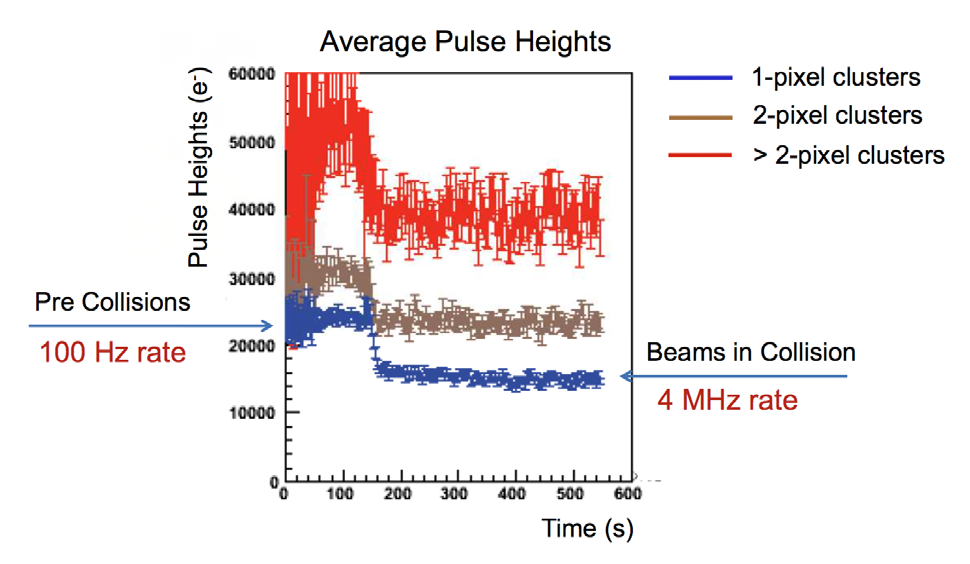
\includegraphics[width=7cm]{plt}
	\end{center}
	\vspace*{-15pt}
	\textbf{Consequences:}
	\begin{itemize}
		\item investigation of the rate effect in scCVD diamonds
		\item using pCVD diamond and prove that they show no rate dependence 
	\end{itemize}
\end{frame}



% ============= RATE ===================
\section{Rate Studies at PSI}
\subsection{General information}
\begin{frame}
	\frametitle{Beam line at Paul Scherrer Institute (PSI)}
	\begin{itemize}
		\setlength{\itemsep}{\fill}
		\item High Intensity Proton Accelerator (HIPA) at PSI (Cyclotron)
		\item \SI{590}{\mega\electronvolt} proton beam with beam current up to \SI{2.4}{\milli\ampere}
		\begin{itemize}
			\vspace*{4pt}
			\item \SI{\sim1.4}{\mega\watt} \ra most powerful proton accelerator in the world
		\end{itemize}
		\item using beam line $\uppi$M1 with \SI{260}{\mega\electronvolt\per c} positive pions ($\uppi^+$)
		\item tunable particle fluxes from \SI{2}{\kilo\hertz\per cm^2} to \SI{10}{\mega\hertz\per cm^2}
	\end{itemize}
	\begin{figure}
		\centering
		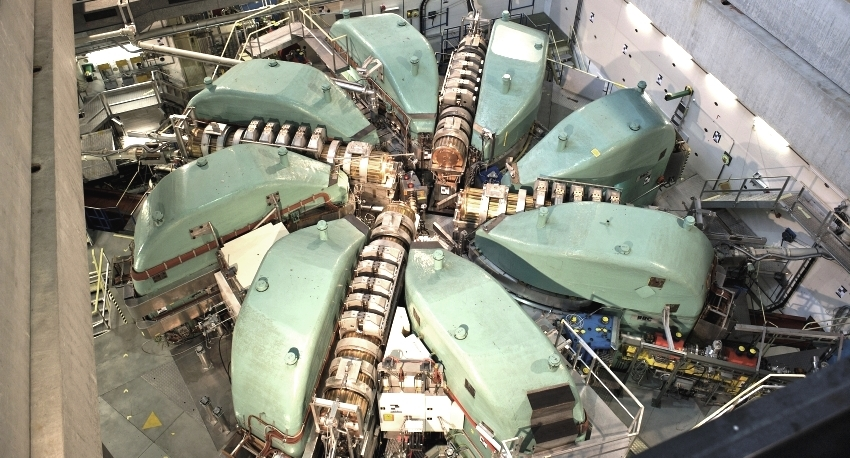
\includegraphics[width=7cm]{cyclotron}
	\end{figure}
\end{frame}
% ============================ new frame ==========================================>
\begin{frame}
	\frametitle{Measurements}
	\begin{itemize}
		\item performing several beam tests starting in $2013$
		\item using a modular self-built beam telescope with two possible setups:
			\begin{itemize}
				\item pad setup (testing whole diamonds as single pad detector)
				\item pixel setup (testing diamond sensors implanted on CMS-Pixel Chips)
			\end{itemize}
		\item investigating several materials and devices
		\begin{itemize}
			\item scCVD pad detectors (reproduce rate effect)
			\item pCVD pad and pixel detectors
			\item very first 3D pixel detector
		\end{itemize}
		\item studying non-irradiated and irradiated devices (up to \SI{1e16}{neq\per cm^2})
	\end{itemize}
	\begin{figure}
		\centering
		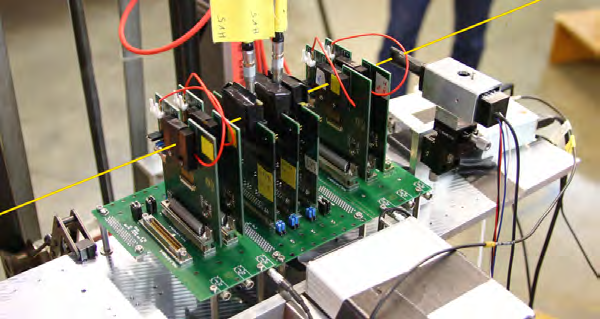
\includegraphics[width=6cm]{pad}
	\end{figure}
\end{frame}
% ============================ new frame ==========================================>
\subsection{Setup}
\begin{frame}
	\frametitle{Setup}
	\begin{figure}
		\centering
		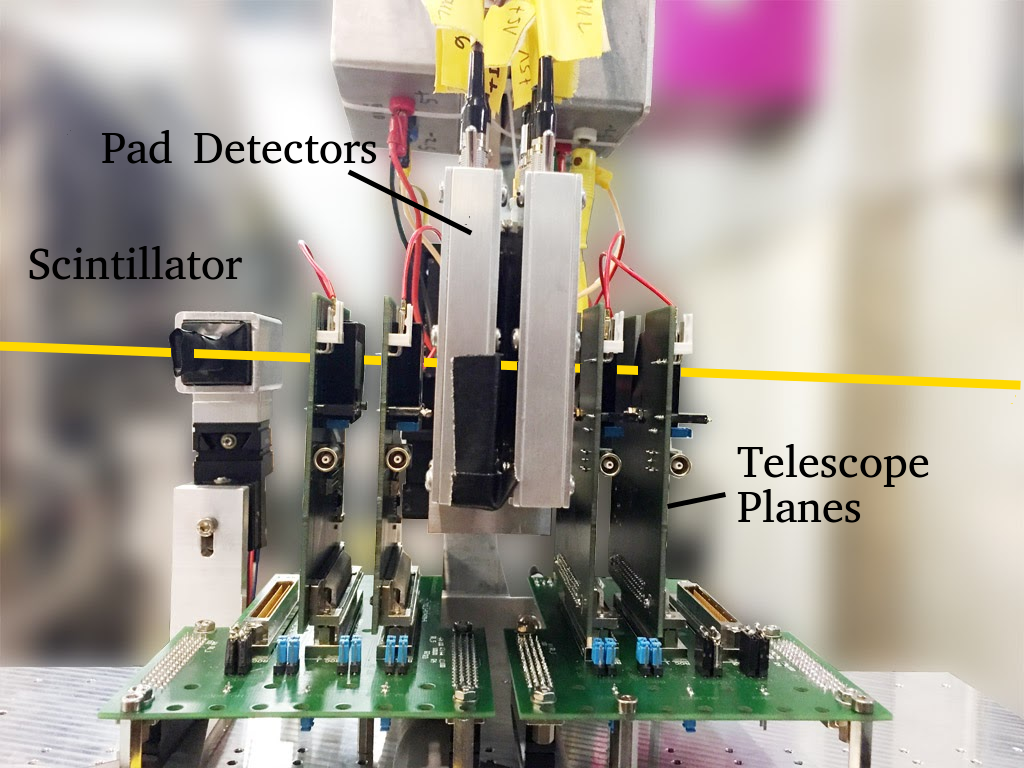
\includegraphics[width=5.5cm]{Setup}
	\end{figure}
	\begin{itemize}
		\setlength{\itemsep}{\fill}
		\item 4 tracking planes with analogue CMS pixel chips
		\item 2 diamond pad detectors
		\item scintillator for precise trigger timing: sigma of \SI{1.3\pm.1}{ns}
		\item resolution: \SI{\sim80x50}{\micro\meter}
	\end{itemize}
\end{frame}
% ============================ new frame ==========================================>
\begin{frame}
	\frametitle{Schematics}
	\begin{figure}
		\centering
		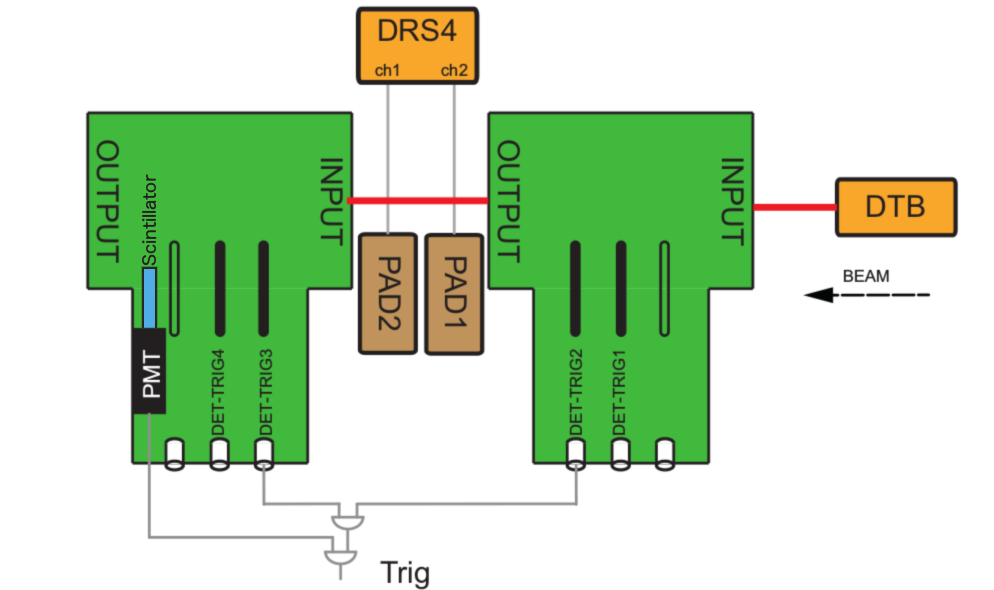
\includegraphics[width=7cm]{SchematicsV2}
	\end{figure}
	\begin{itemize}
		\setlength{\itemsep}{\fill}
		\item using PSI DRS4 Evaluation Board as digitizer for the pad waveforms
		\item using Digital Test Board (DTB) and pXar software for the telescope readout
		\item global trigger as coincidence of fastOR self trigger and scintillator signal
		\item EUDAQ as DAQ framework
	\end{itemize}
\end{frame}
% ============================ new frame ==========================================>
\begin{frame}
	\frametitle{DAQ}
	\begin{figure}
		\centering
		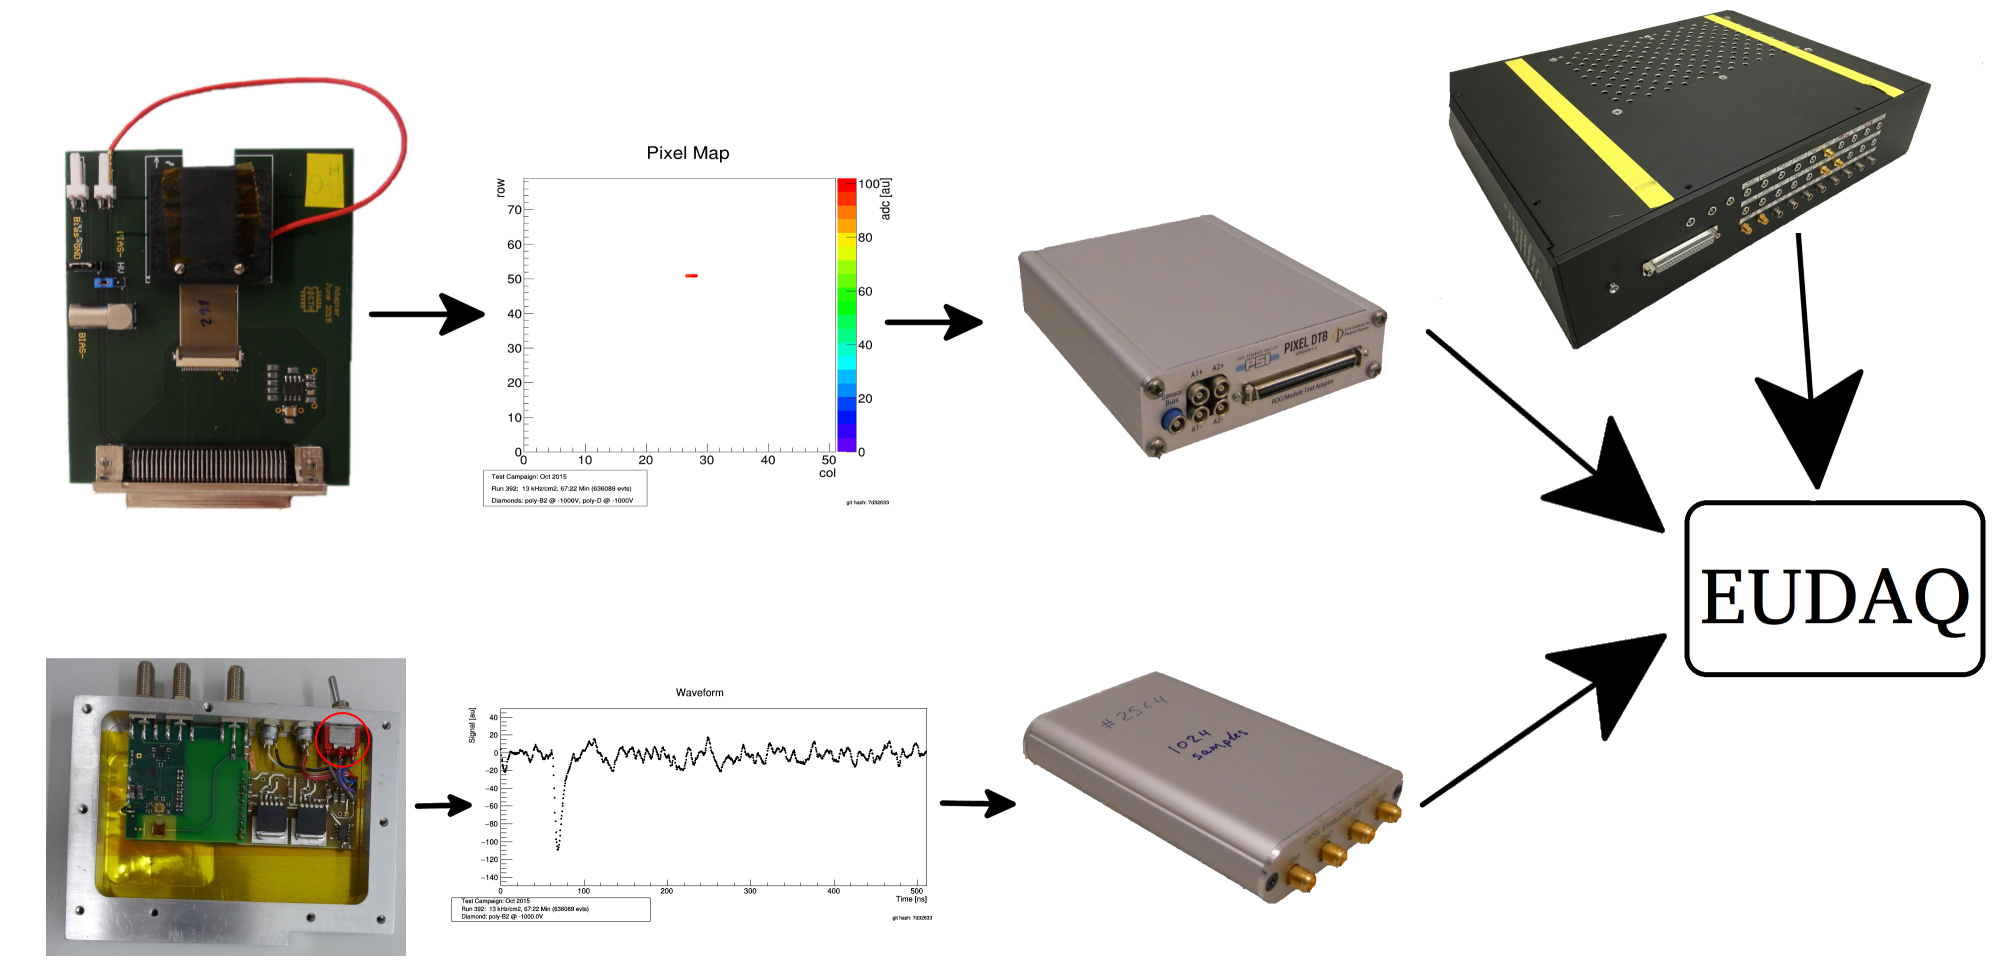
\includegraphics[width=.8\textwidth]{Intro}
	\end{figure}
	\begin{itemize}
		\item custom-built trigger unit to process the single triggers and provide global one for all devices
		\item saving event based data stream as binary file using EUDAQ
	\end{itemize}
\end{frame}
% ============================ new frame ==========================================>
\subsection{Analysis and Results}
\begin{frame}
	\frametitle{Waveforms}
	\vspace*{-20pt}
	\begin{center}
		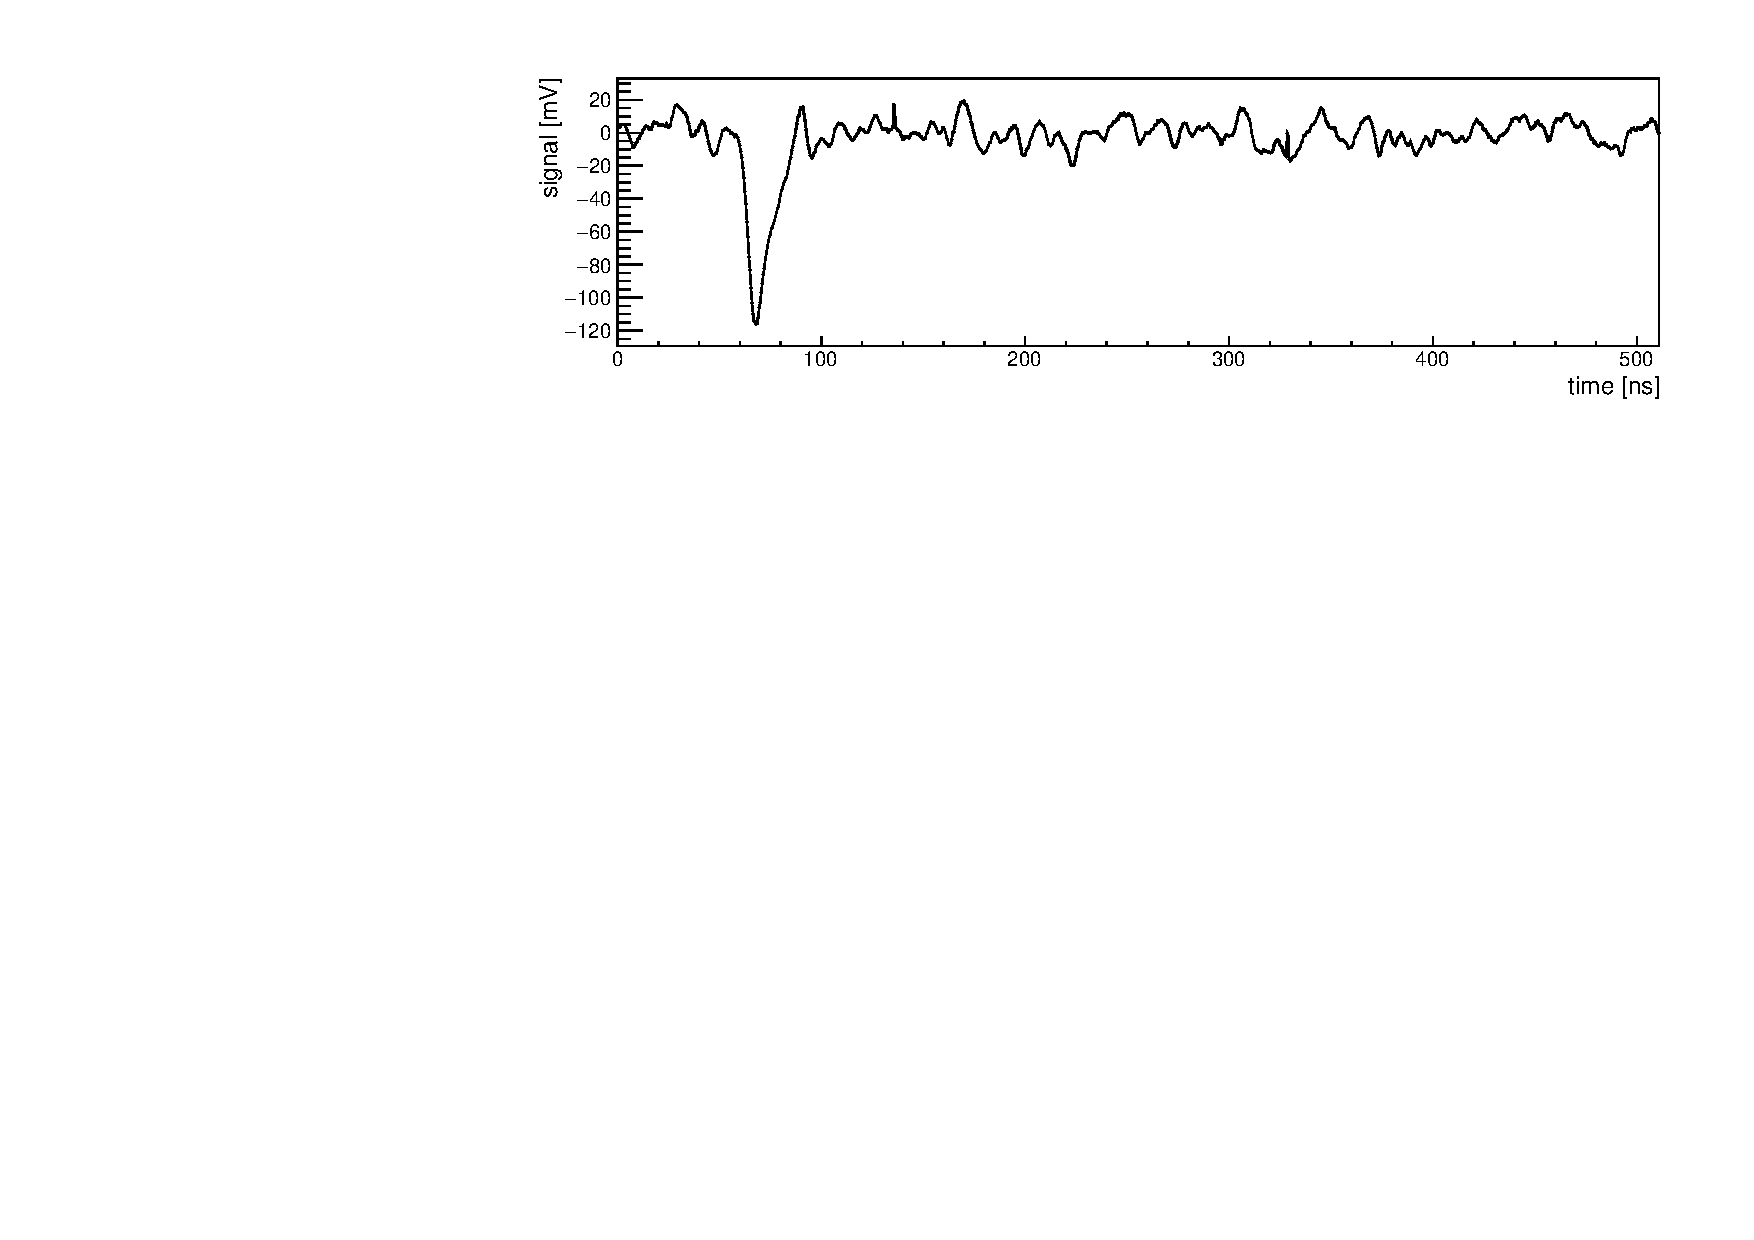
\includegraphics[angle=270, width=.7\textwidth]{SignalWaveform}\\
		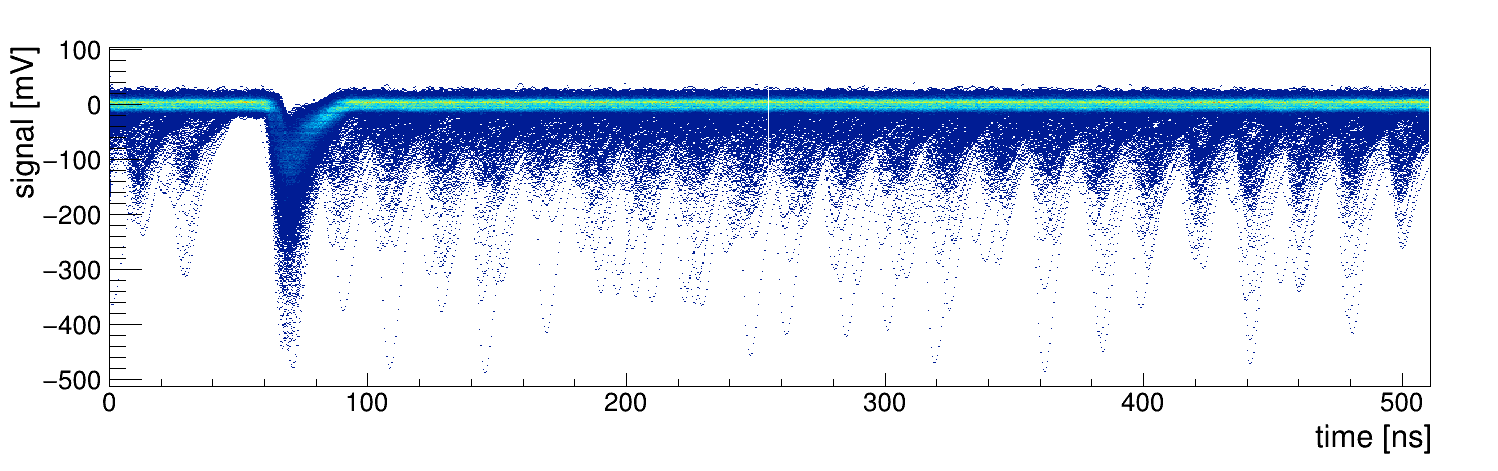
\includegraphics[width=.7\textwidth]{SignalWaveforms5000}
	\end{center}
	\begin{itemize}
		\item most frequented peak (\SI{\sim70}{ns}): triggered signal
		\item other peaks originate from other buckets ($\rightarrow$ resolve beam structure of \SI{\approx19.7}{ns})
		\item system does not allow signals in pre-signal bucket due to fastOR trigger deadtime
	\end{itemize}
\end{frame}
% ============================ new frame ==========================================>
\begin{frame}
	\frametitle{Pulse Height Calculation}
	\begin{center}
		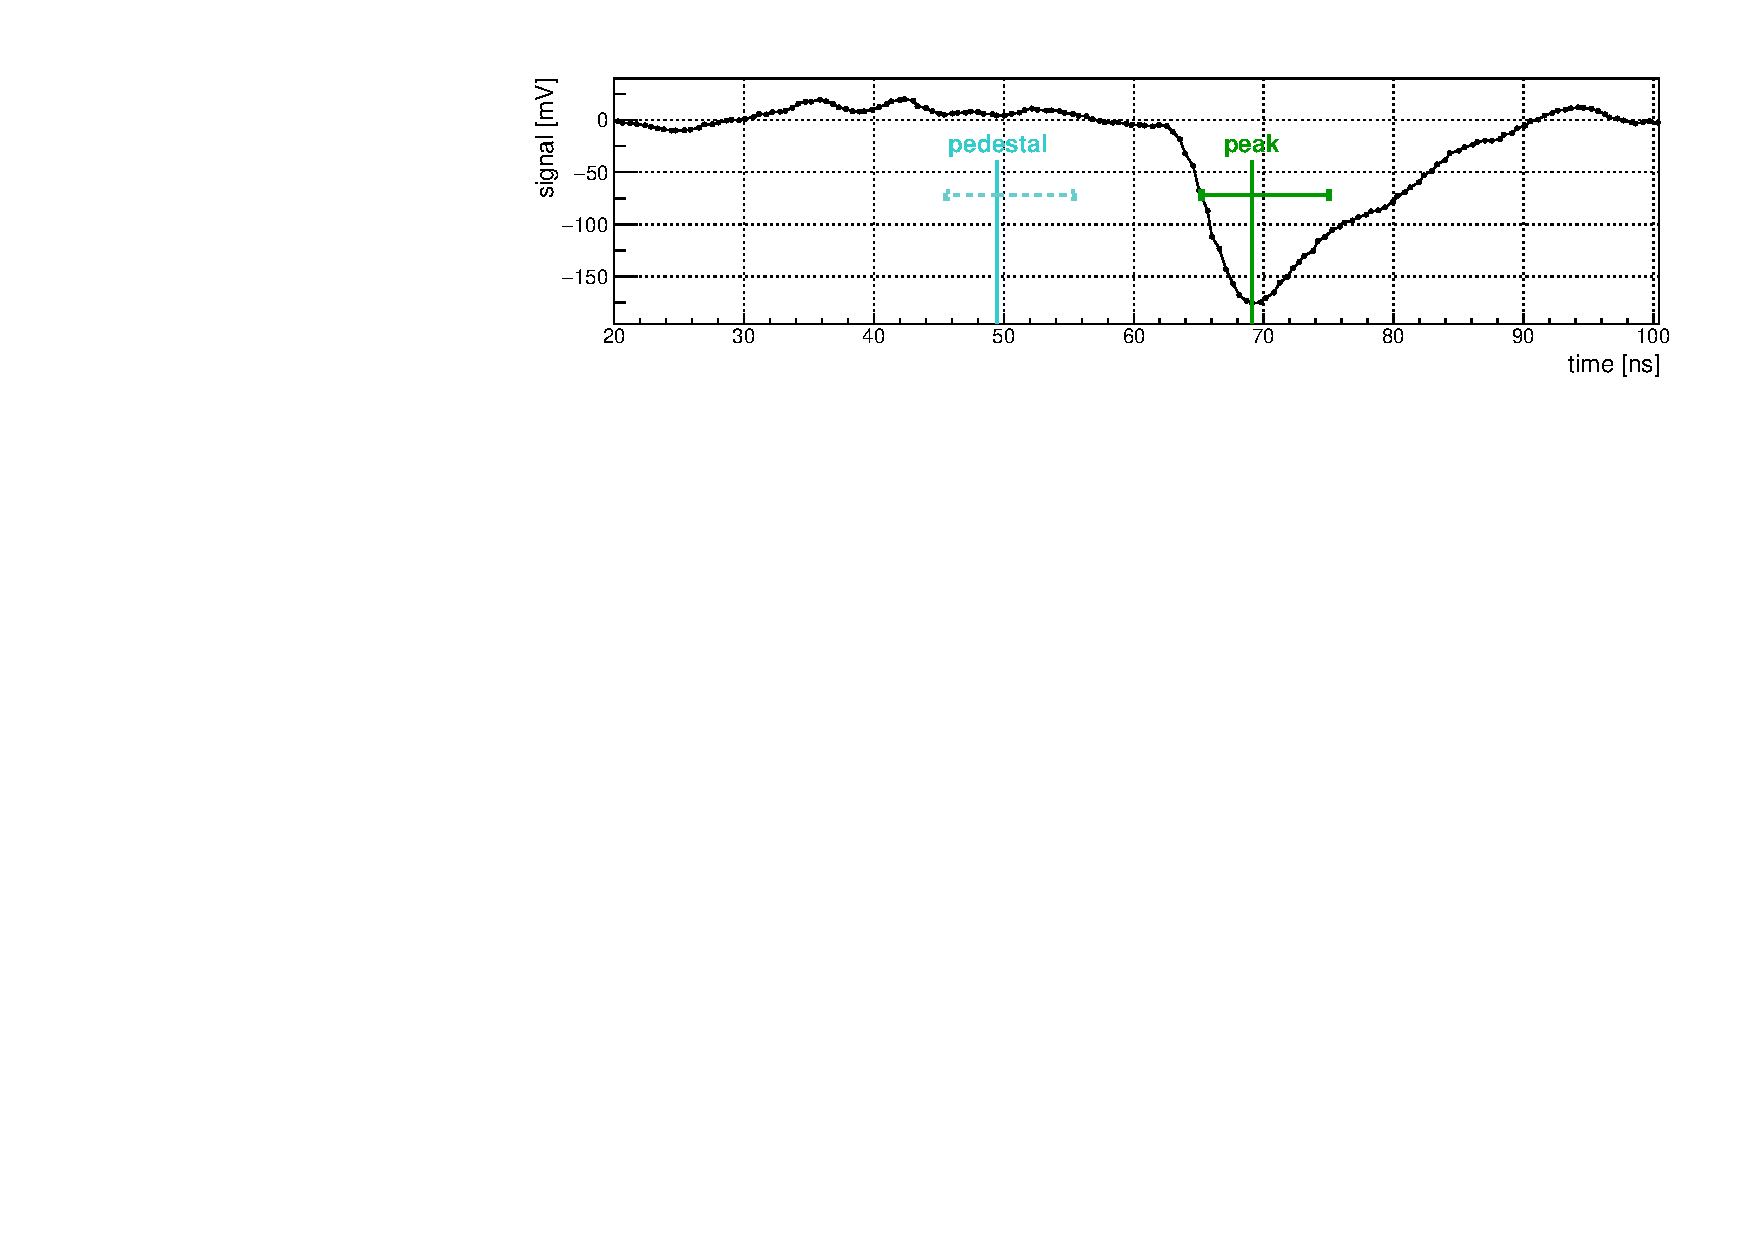
\includegraphics[angle=270, width=.8\textwidth]{intpeaks}\\
	\end{center}
	\begin{itemize}
		\setlength{\itemsep}{\fill}
		\item finding the peak in the signal region
		\item integrating the signal in time fixed asymmetric integral around peak
		\item same integration for pedestal (base line $\rightarrow$ noise)
		\item optimising the integral width by highest SNR (Integral / Pedestal Sigma)
		\item subtracting the pedestal from the signal integral on event-wise basis 
	\end{itemize}
\end{frame}
% ============================ FRAME 18 ==========================================>
\begin{frame}
	\frametitle{Pulse Height Distribution and Signal Maps}
	\vspace*{-7.5pt}
	\def \sp {0.65\textwidth}
	\begin{figure}
		\centering
		\begin{subfigure}{0.45\textwidth} 
			\centering 
			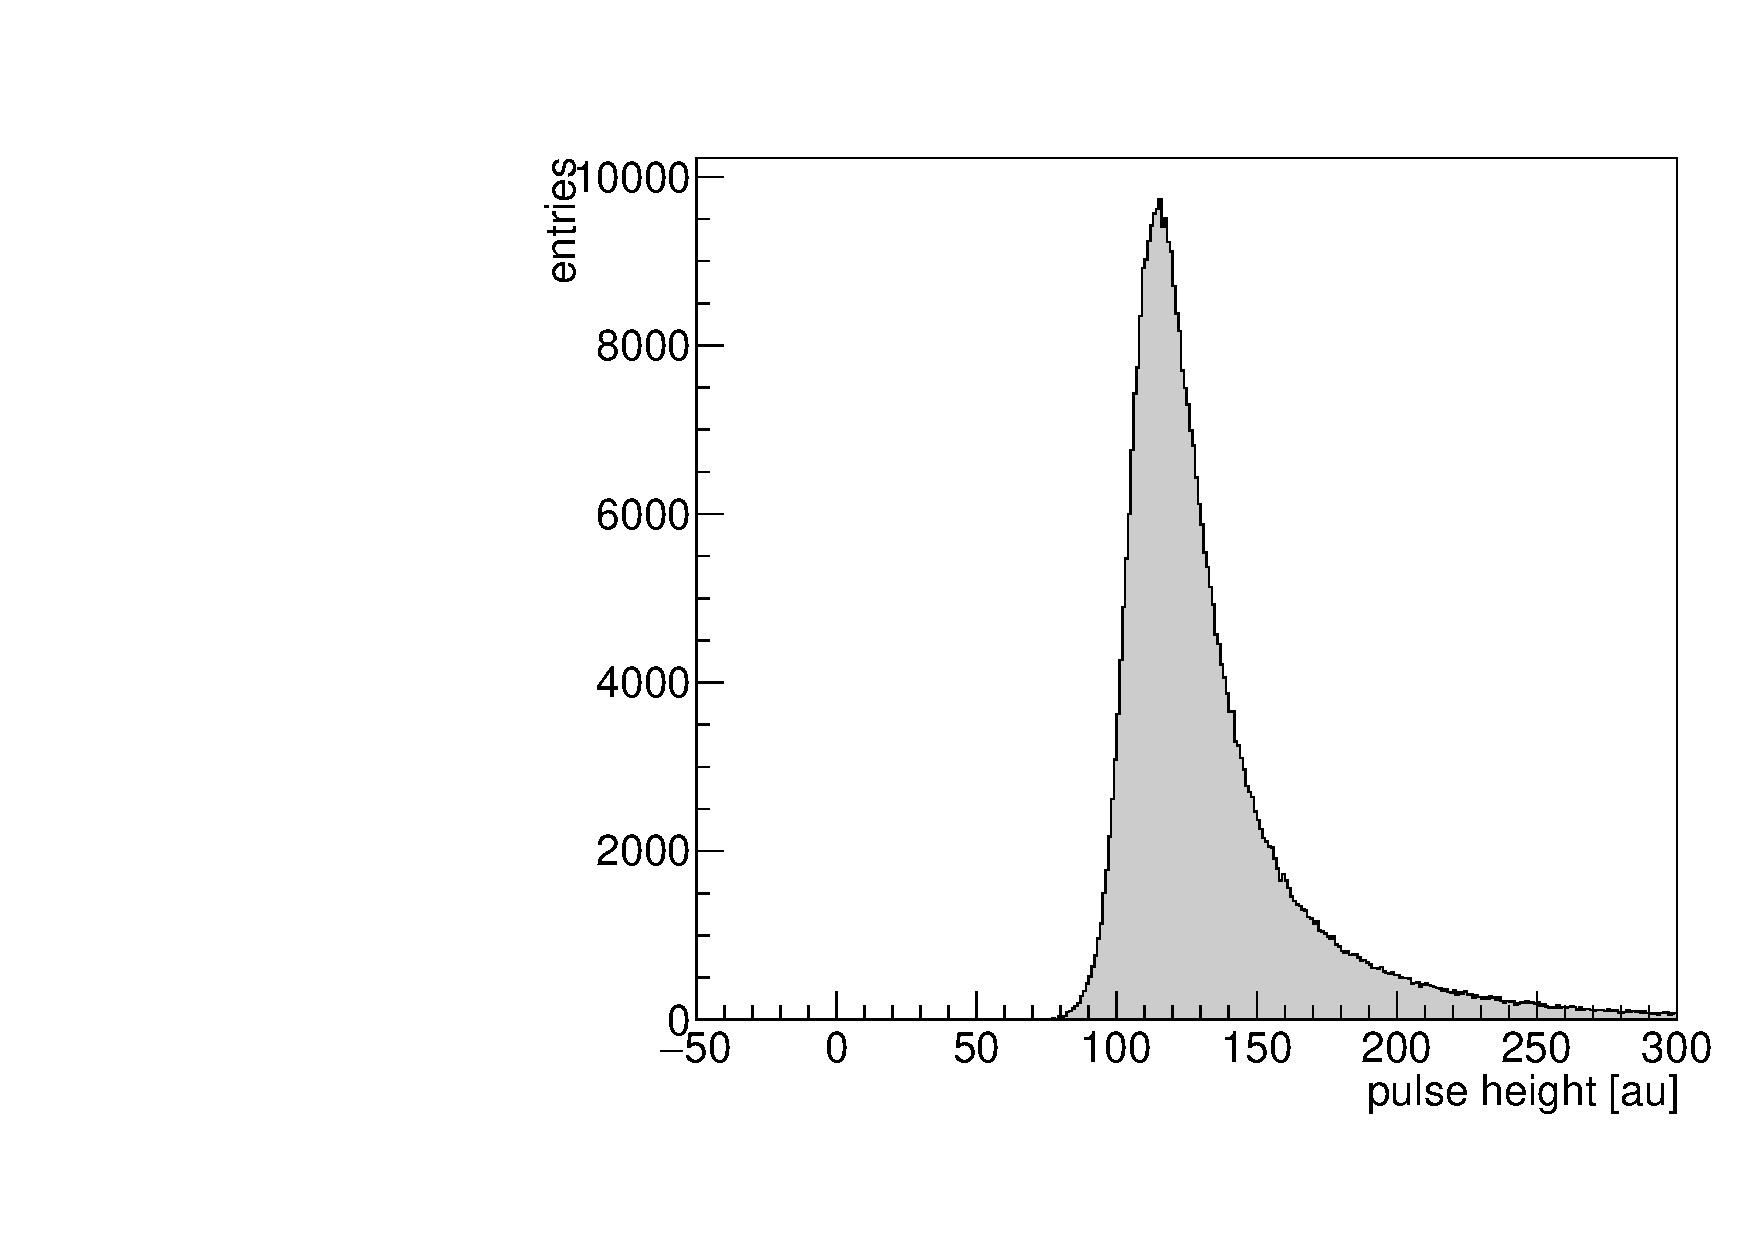
\includegraphics[angle=270, width=\sp]{sDisto}
		\end{subfigure}
		\begin{subfigure}{0.45\textwidth} 
			\centering 
			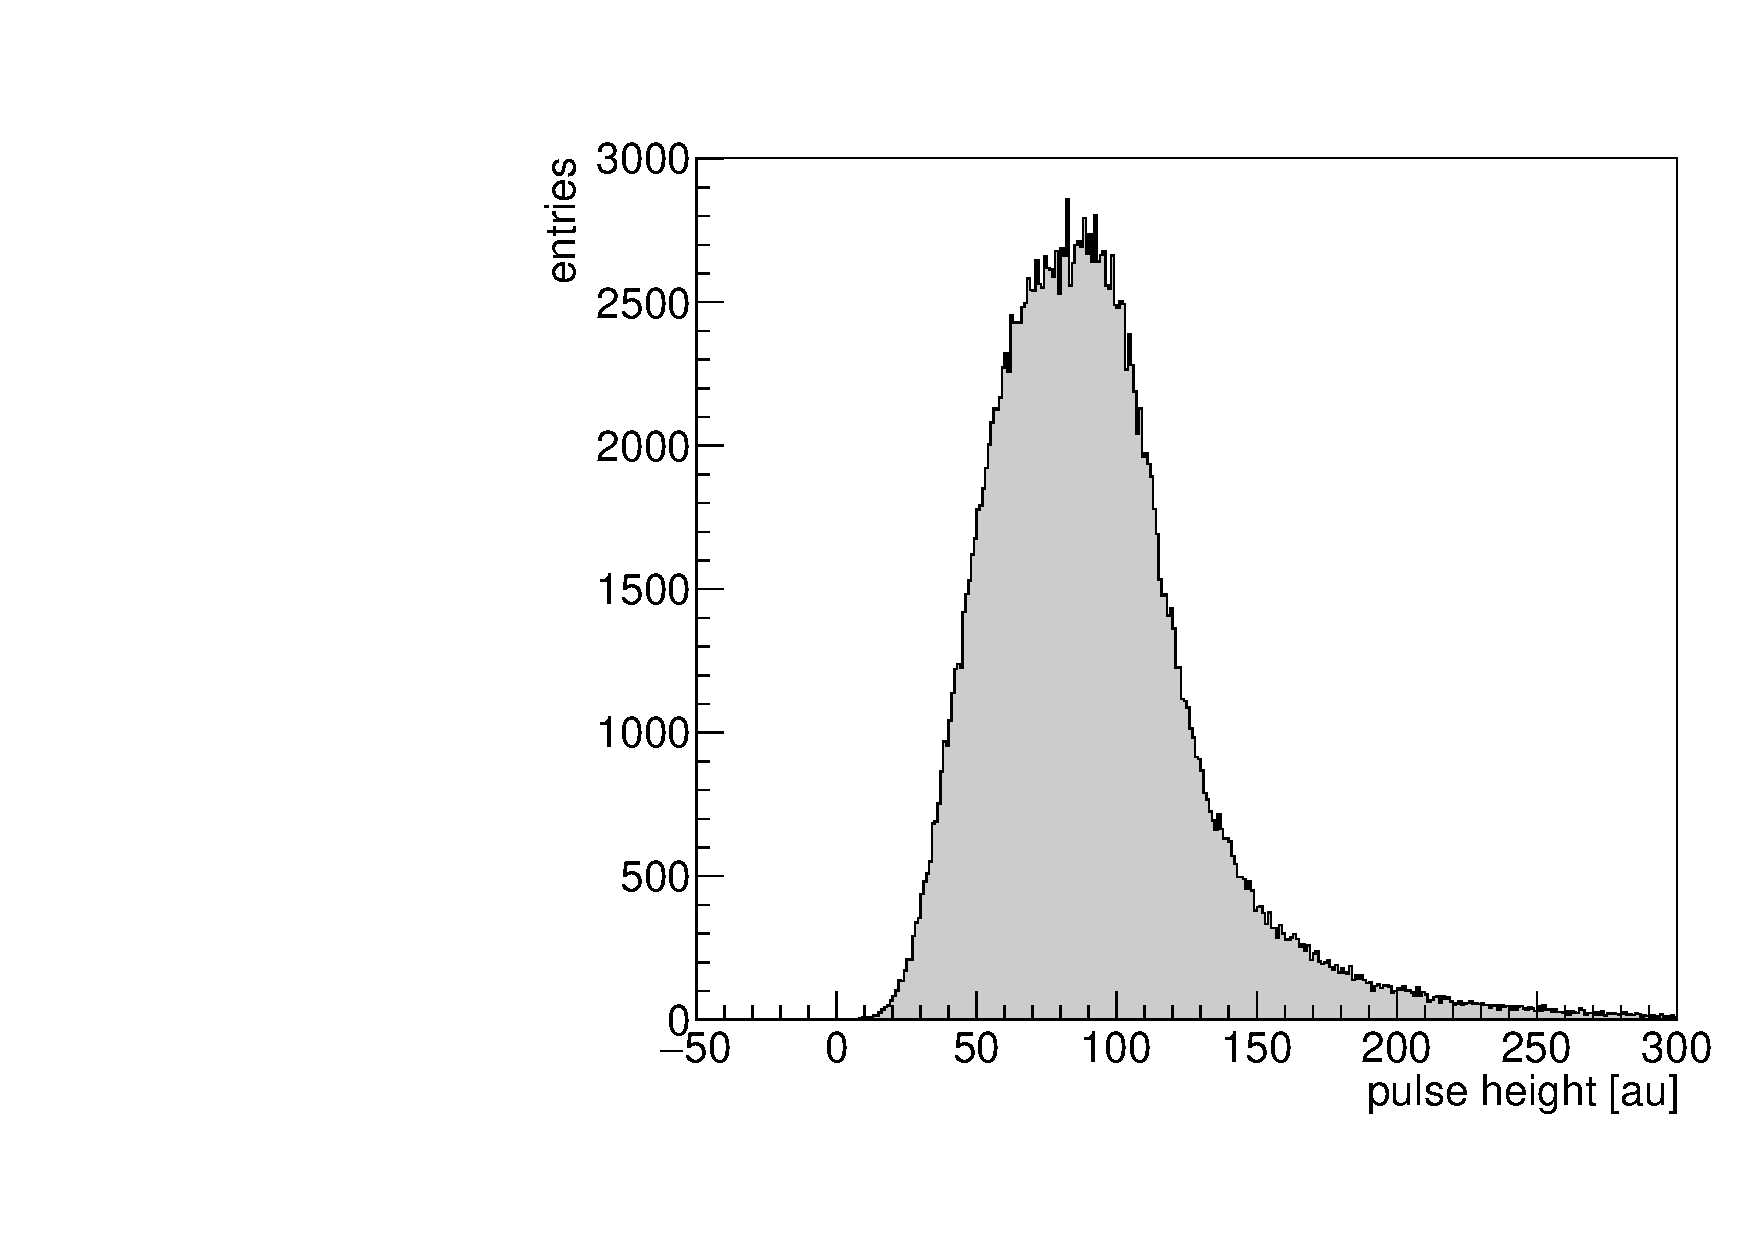
\includegraphics[angle=270, width=\sp]{pDisto}
		\end{subfigure}
	\end{figure}
	\vspace*{-15pt}
	\begin{figure}
	\centering
		\begin{subfigure}{0.45\textwidth} 
			\centering 
			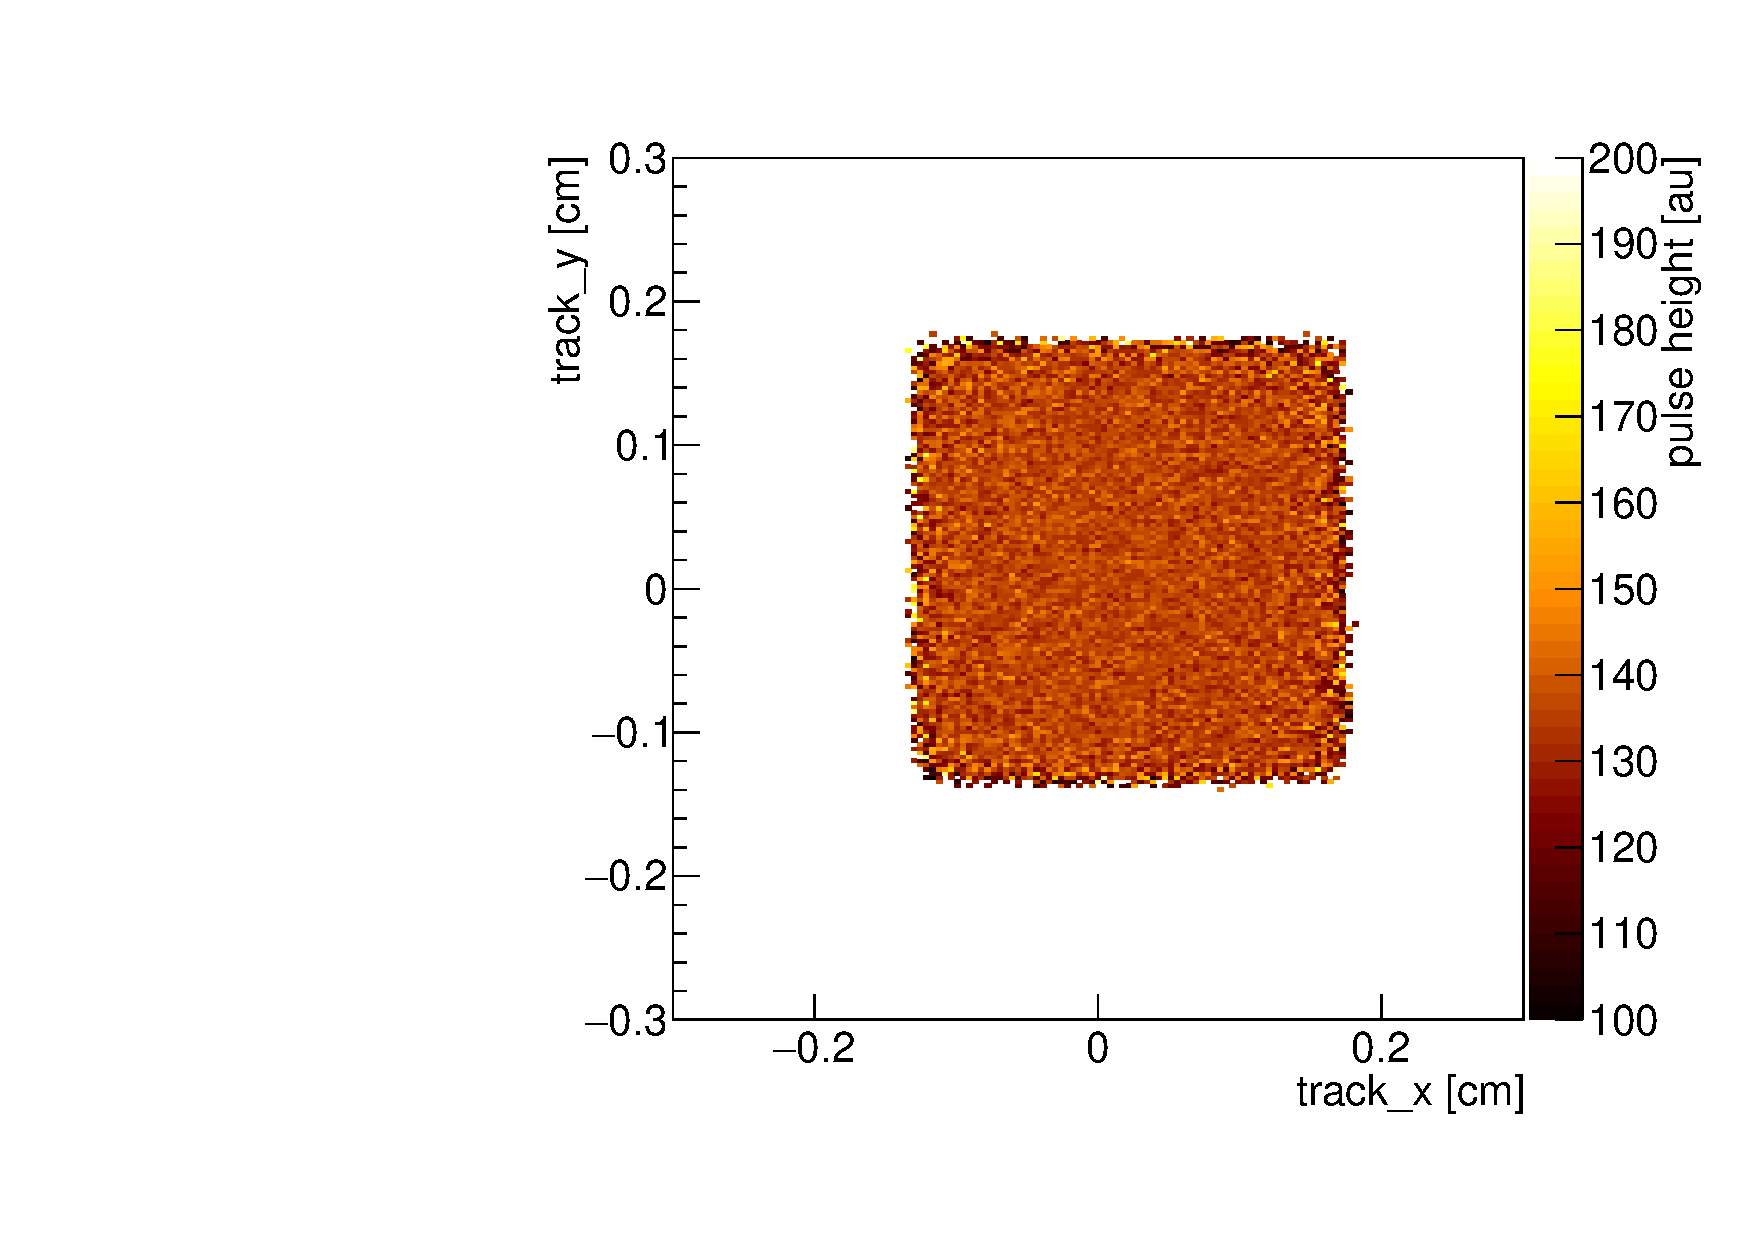
\includegraphics[angle=270, width=\sp]{sSigMap}
			\caption{single-crystalline}
		\end{subfigure}
		\begin{subfigure}{0.45\textwidth} 
			\centering 
			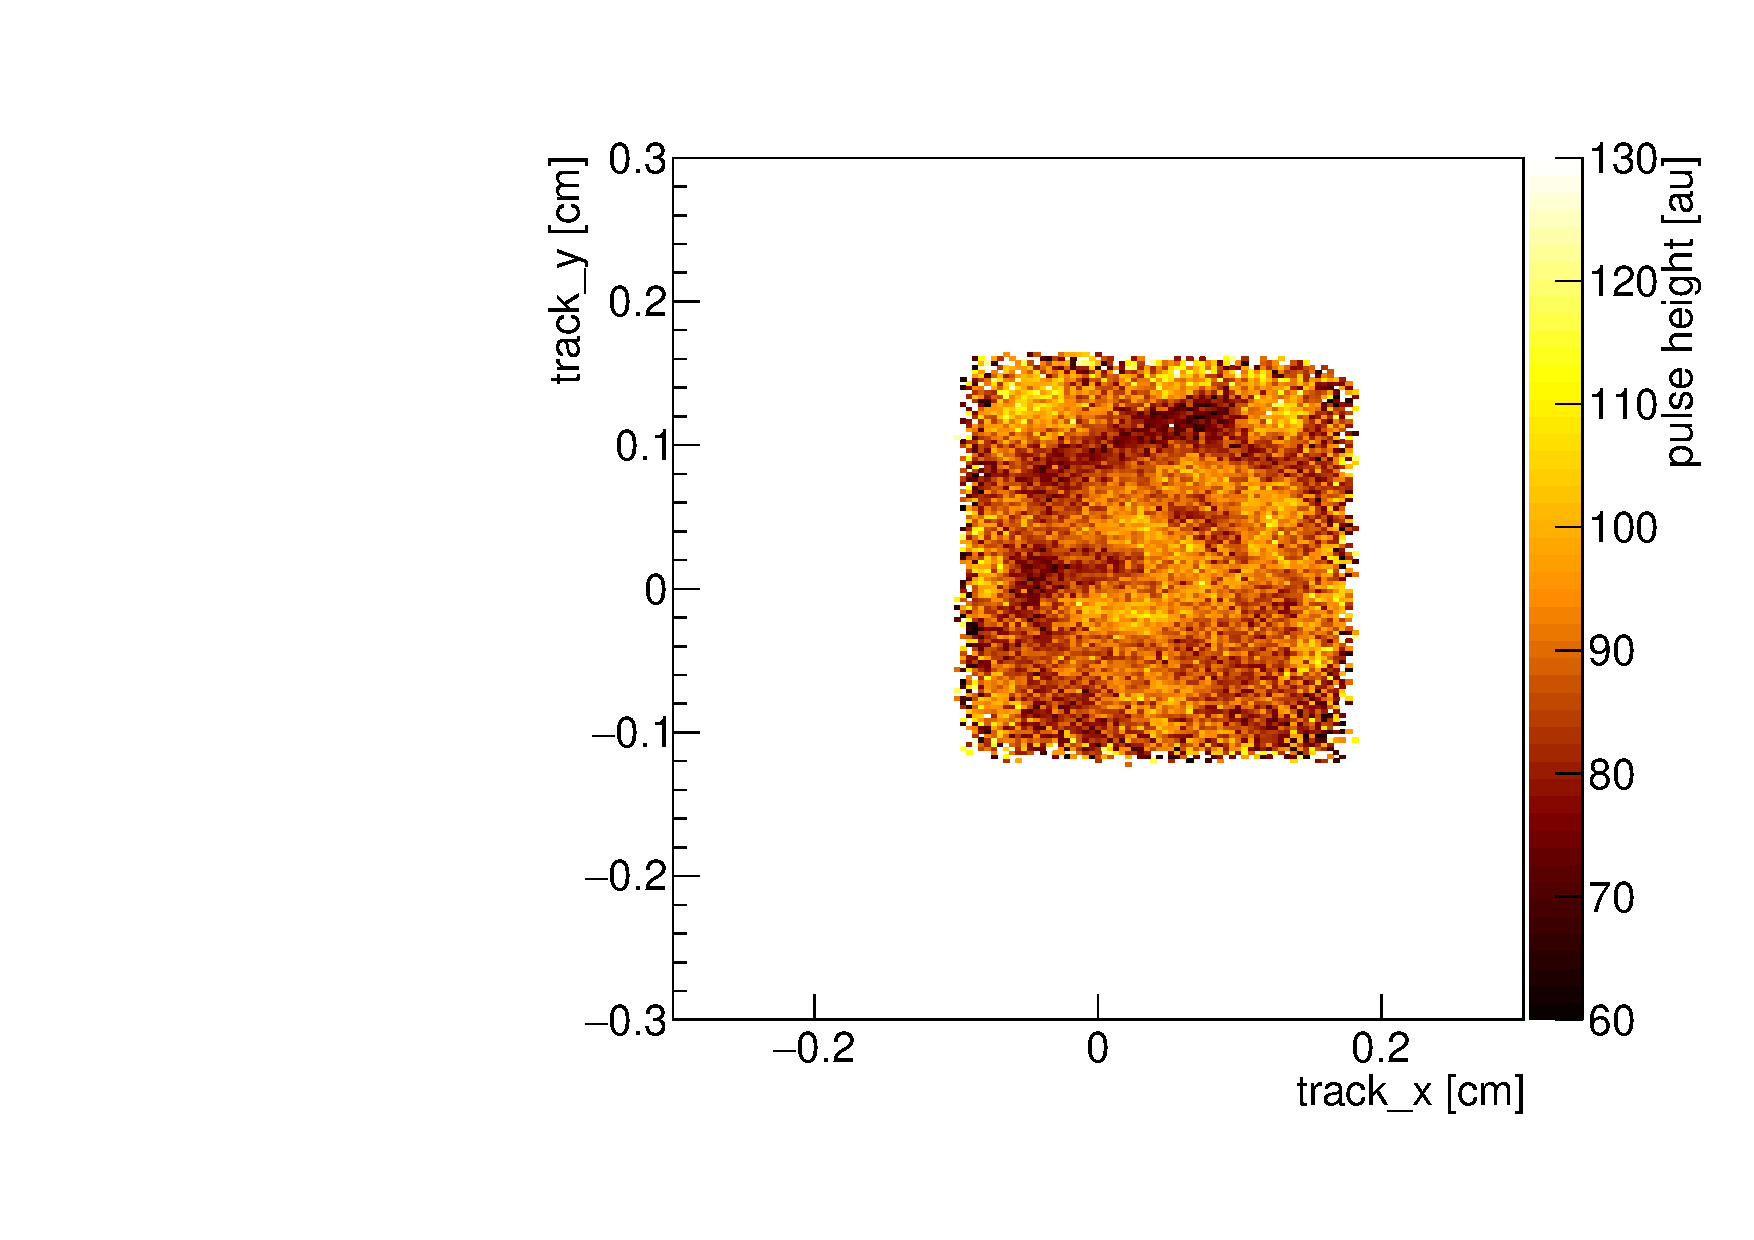
\includegraphics[angle=270, width=\sp]{pSigMap}
			\caption{poly-crystalline}
		\end{subfigure} 
	\end{figure}
\end{frame}
% ============================ new frame ==========================================>
\begin{frame}
	\frametitle{Signal vs. Particle Flux}
	\begin{minipage}[c][.75\textheight]{.5\textwidth}
		\begin{itemize}
			\setlength{\itemsep}{\fill}
			\item after all analysis steps: look for rate dependence of pCVD diamonds
			\item found diamond pad detectors that show no or very little dependence on rate
			\item no dependence up to \SI{1e16}{neq\per cm^2}
			\item large systematic errors due to reproducibility
		\end{itemize}
		\vspace*{3pt}
		\textbf{To do:}
		\begin{itemize}
			\setlength{\itemsep}{\fill}
			\item test higher irradiated samples
			\item improve reproducibility
			\item prove the same for pixel detectors
		\end{itemize}
	\end{minipage}
	\hspace*{5pt}
	\begin{minipage}{.45\textwidth}
		\begin{figure}
			\centering
			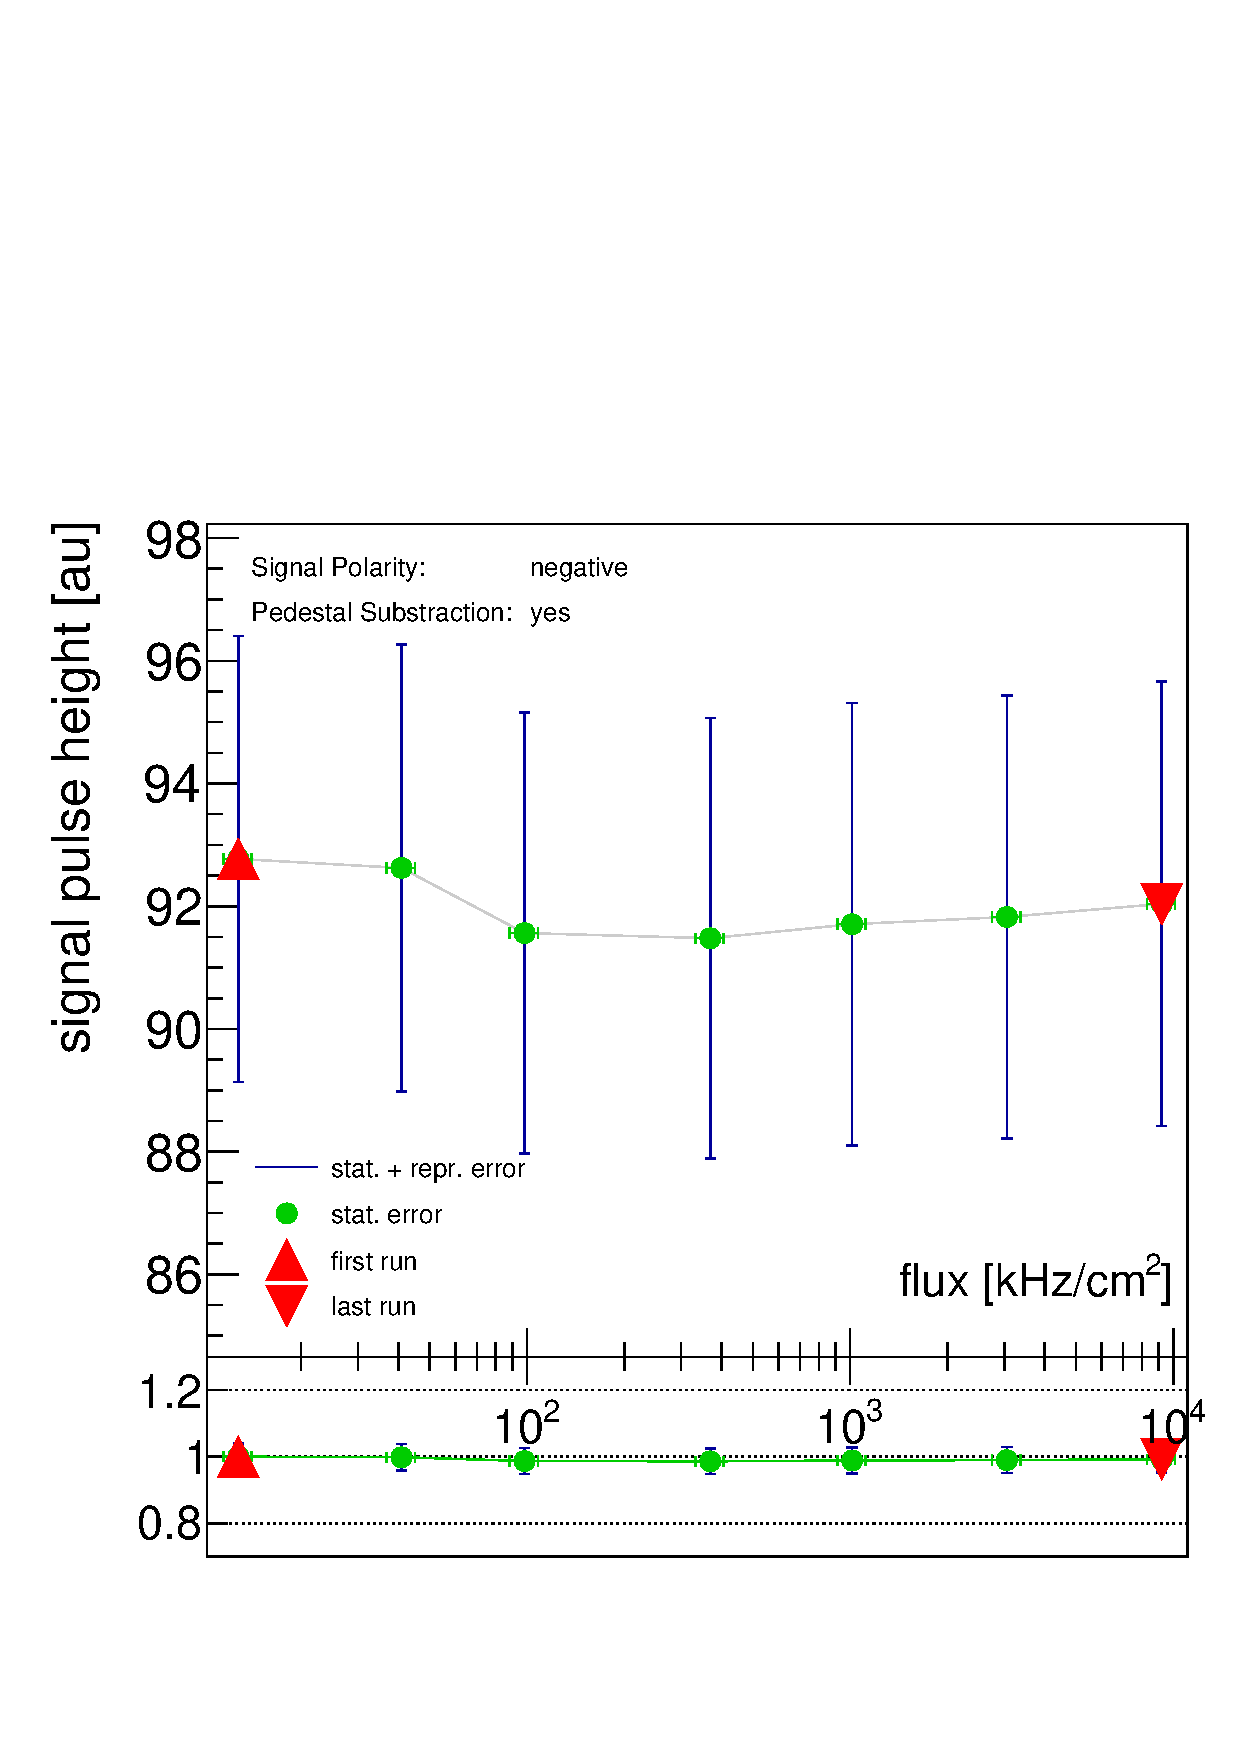
\includegraphics[width=\textwidth]{rateplot}
		\end{figure}
	\end{minipage}
\end{frame}


% ============= 3D =====================
\section{3D Detectors at CERN}
\subsection{Working Principle}
\begin{frame}
	\frametitle{Working Principle}
	\begin{itemize}
		\setlength{\itemsep}{\fill}
		\item insert electrodes perpendicular to the plane
		\begin{itemize}
			\item reduce drift distance
			\item increase collected charge in detectors with limited mean free path %(e.g. irradiated devices)
		\end{itemize}
		\item one readout electrode surrounded by four bias electrodes
		\item in diamond electrodes formed with a pulsed laser
		\begin{itemize}
			\item transition of diamond to conducting material (i.a. graphitic material)
		\end{itemize}
	\end{itemize}
	\begin{figure}
		\centering
		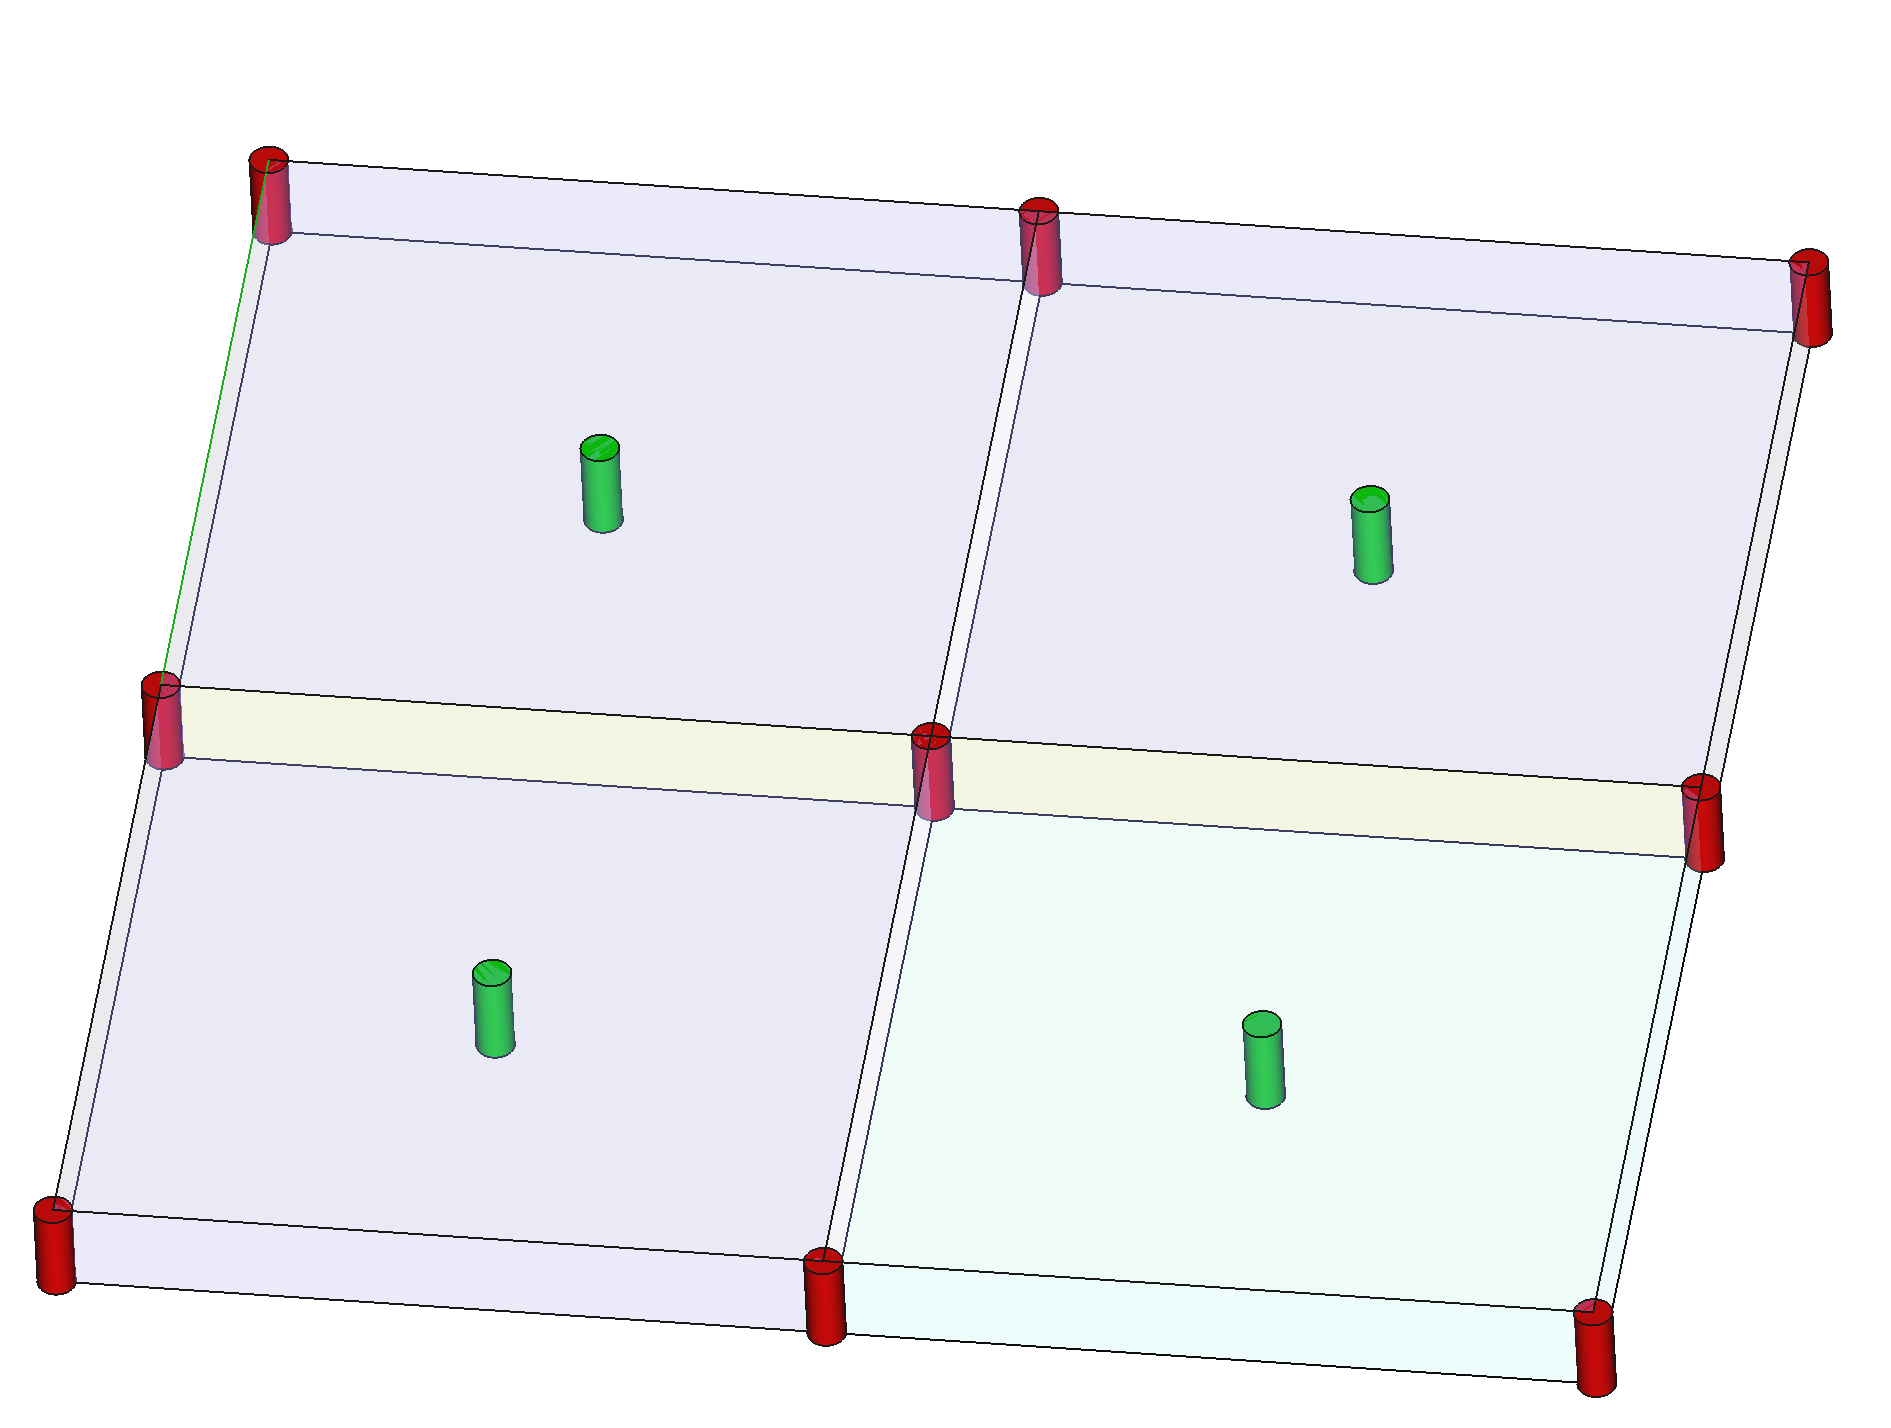
\includegraphics[width=5cm]{3DScheme}
		\caption{array of four 3D cells, bias electrodes in red, readout electrodes in green}
	\end{figure}
\end{frame}
% ============================ new frame ==========================================>
\subsection{Beam Tests at CERN}
\begin{frame}
	\frametitle{Beam Tests at CERN}
	\begin{itemize}
		\setlength{\itemsep}{\fill}
		\item using more than 20 years old fixed telescope at SPS at CERN
		\item testing multiple 3D strip detectors
		\item basic working principle has been proven
		\item full charge collection not yet reached in pCVD
		\item improve fabrication technique
	\end{itemize}
	\begin{figure}
		\centering
		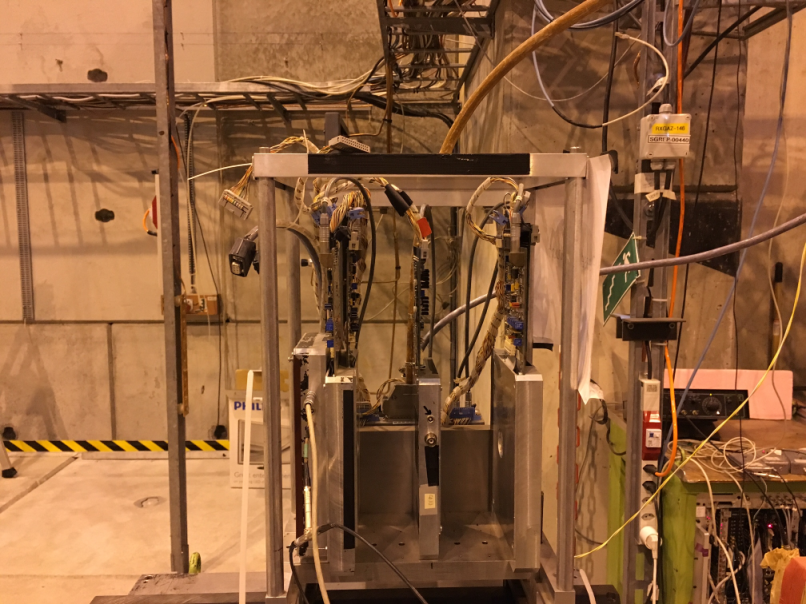
\includegraphics[width=4.5cm]{3DTelescope}
		\caption{Strassbourg Telescope}
	\end{figure}
\end{frame}

% ============= EDGE TCT ===============
% \section{Edge TCT}
% \subsection{Bla}
\begin{frame}
	nada
\end{frame}

% ============= CONCLUSION =============
\section{Conclusion}
\subsection{Bla}
\begin{frame}
	nada
\end{frame}

% DOCUMENT END
\end{document}

